\documentclass{standalone}

\usepackage{tikz}
\usetikzlibrary{calc}

\def \D { (0,0), (3,0), (6,0), (9,0), (2,1), (5,1), (1,2), (10,2), (3,3), (6,3), (9,3), (8,4), (11,4), (4,5), (7,5), (0,6), (3,6), (2,7), (5,7), (8,7), (1,8), (10,8), (6,9), (9,9), (2,10), (5,10), (8,10), (11,10) }

\def \A { 
	(0,0), (9,0), (2,1), (5,1), (10,2), (3,3), (6,3), (4,5), (7,5), (0,6),  (5,7), (8,7), (1,8), (10,8), (2,10), (5,10), (8,10), (0,12), (9,12), (2,13), (5,13), (10,14), (3,15), (6,15), (4,17), (7,17), (0,18),  (5,19), (8,19), (1,20), (10,20) }

\def \B { (3,0), (6,0), (2,1), (10,2), (9,3), (8,4), (4,5), (3,6), (2,7), (10,8), (6,9), (9,9),
(3,12), (6,12), (2,13), (10,14), (9,15), (8,16), (4,17), (3,18), (2,19), (10,20), (6,21), (9,21) }

\tikzset{
    vvertex/.style= 
    	{shape=circle, draw, line width=1mm, minimum size=5mm, fill=white},
    }

\begin{document}
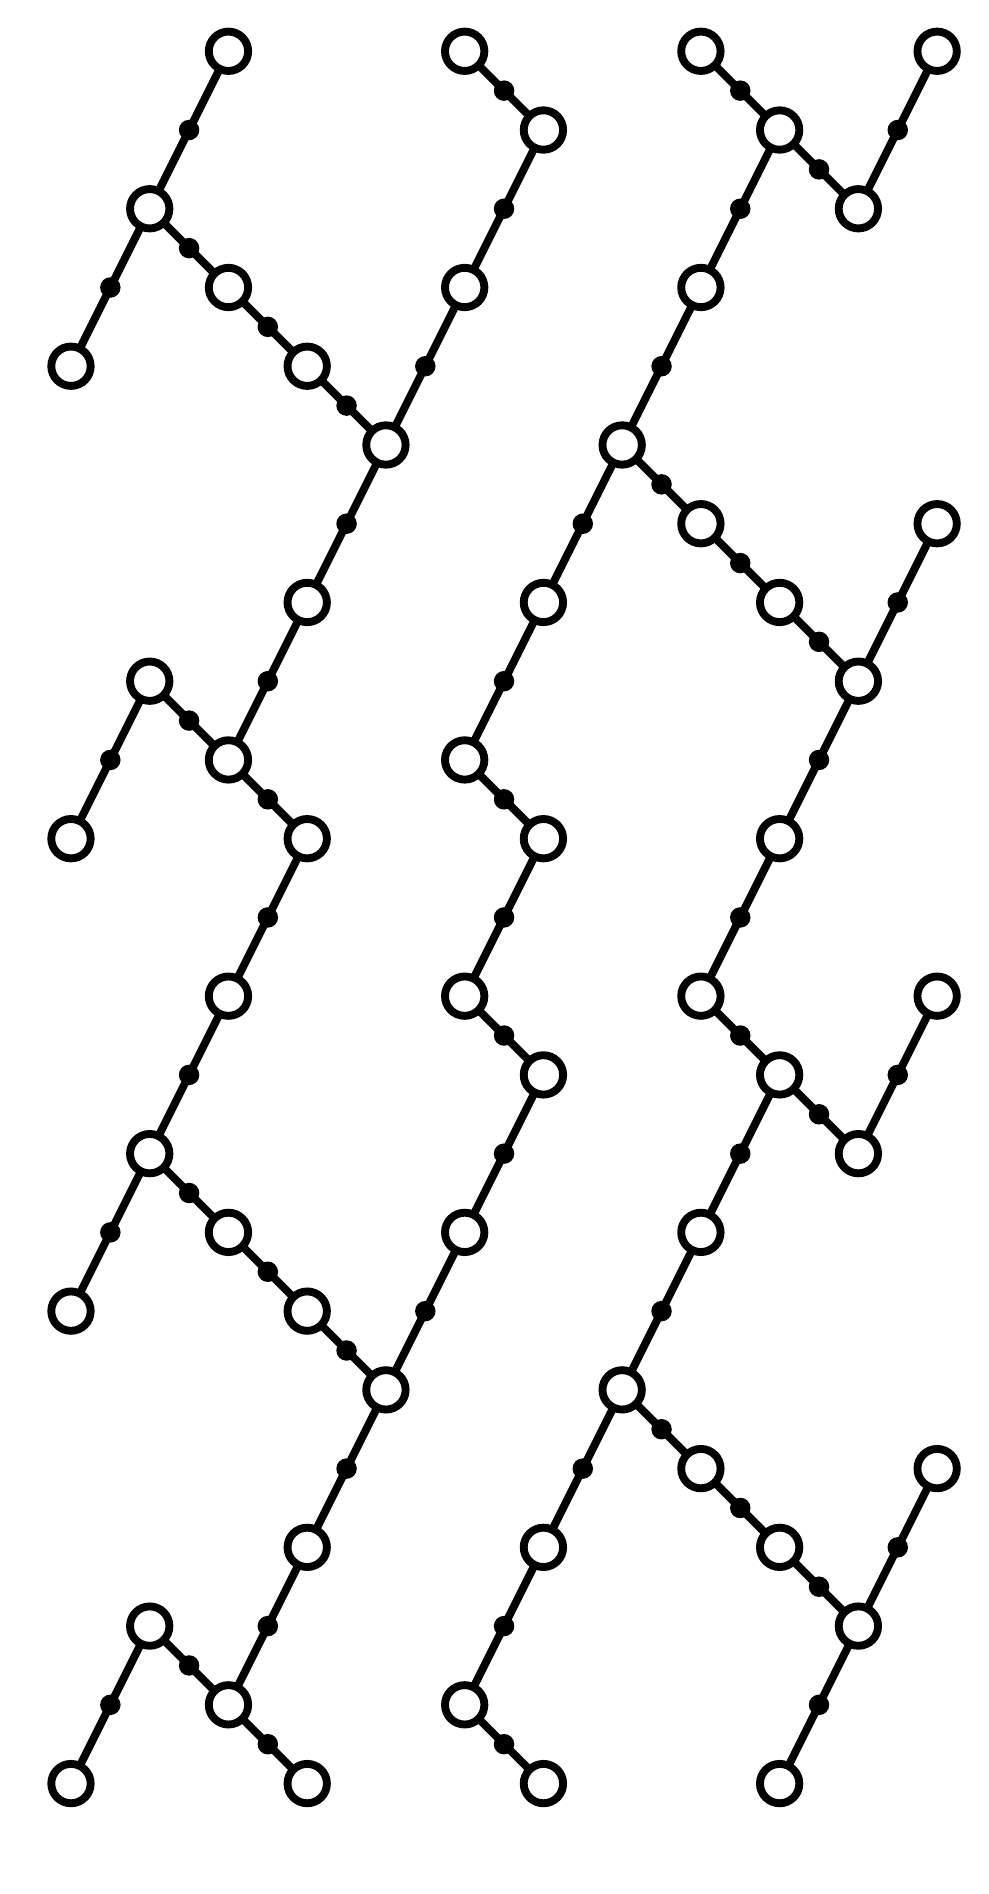
\begin{tikzpicture}
%\draw[help lines, black!15] (0,0) grid (12,24);
\foreach \a in \A
    {\draw[black, line width=1mm]
    	\a++(0.5,1) -- +(1,2);
	 \fill[black,]
    	\a++(1,2) circle (1.3mm);
    } 
\foreach \a in \B
    {\draw[black, line width=1mm]
    	\a++(0.5,1) -- +(-1,1);
	 \fill[black,]
    	\a++(0,1.5) circle (1.3mm);
    }
\foreach \a in \D
    {\node[vvertex, shift={(0.5,1)}] at \a{};
	 \node[vvertex, shift={(0.5,13)}] at \a{}; 
    };

%\draw[black, line width=1mm] (0,0) rectangle (12,24);
\end{tikzpicture}
\end{document}